\documentclass[12pt]{scrreprt}
\usepackage[utf8]{inputenc}
\usepackage{tikz}
\usetikzlibrary{arrows,shapes,positioning,shadows,trees,calc}
\usepackage{caption}
\newcommand{\species}[2]{\emph{#1 #2}}
\tikzset{
  basic/.style  = {draw, drop shadow, font=\sffamily, rectangle},
  root/.style = {basic, rounded corners=2pt, thin, align=center, fill=gray!20},
  level 2/.style = {basic, rounded corners=6pt, thin,align=center, fill=white,
  text width=15em},
  level 3/.style = {basic, thin, align=center, fill=white, minimum height=1cm, text width=8em}
}
\begin{document}
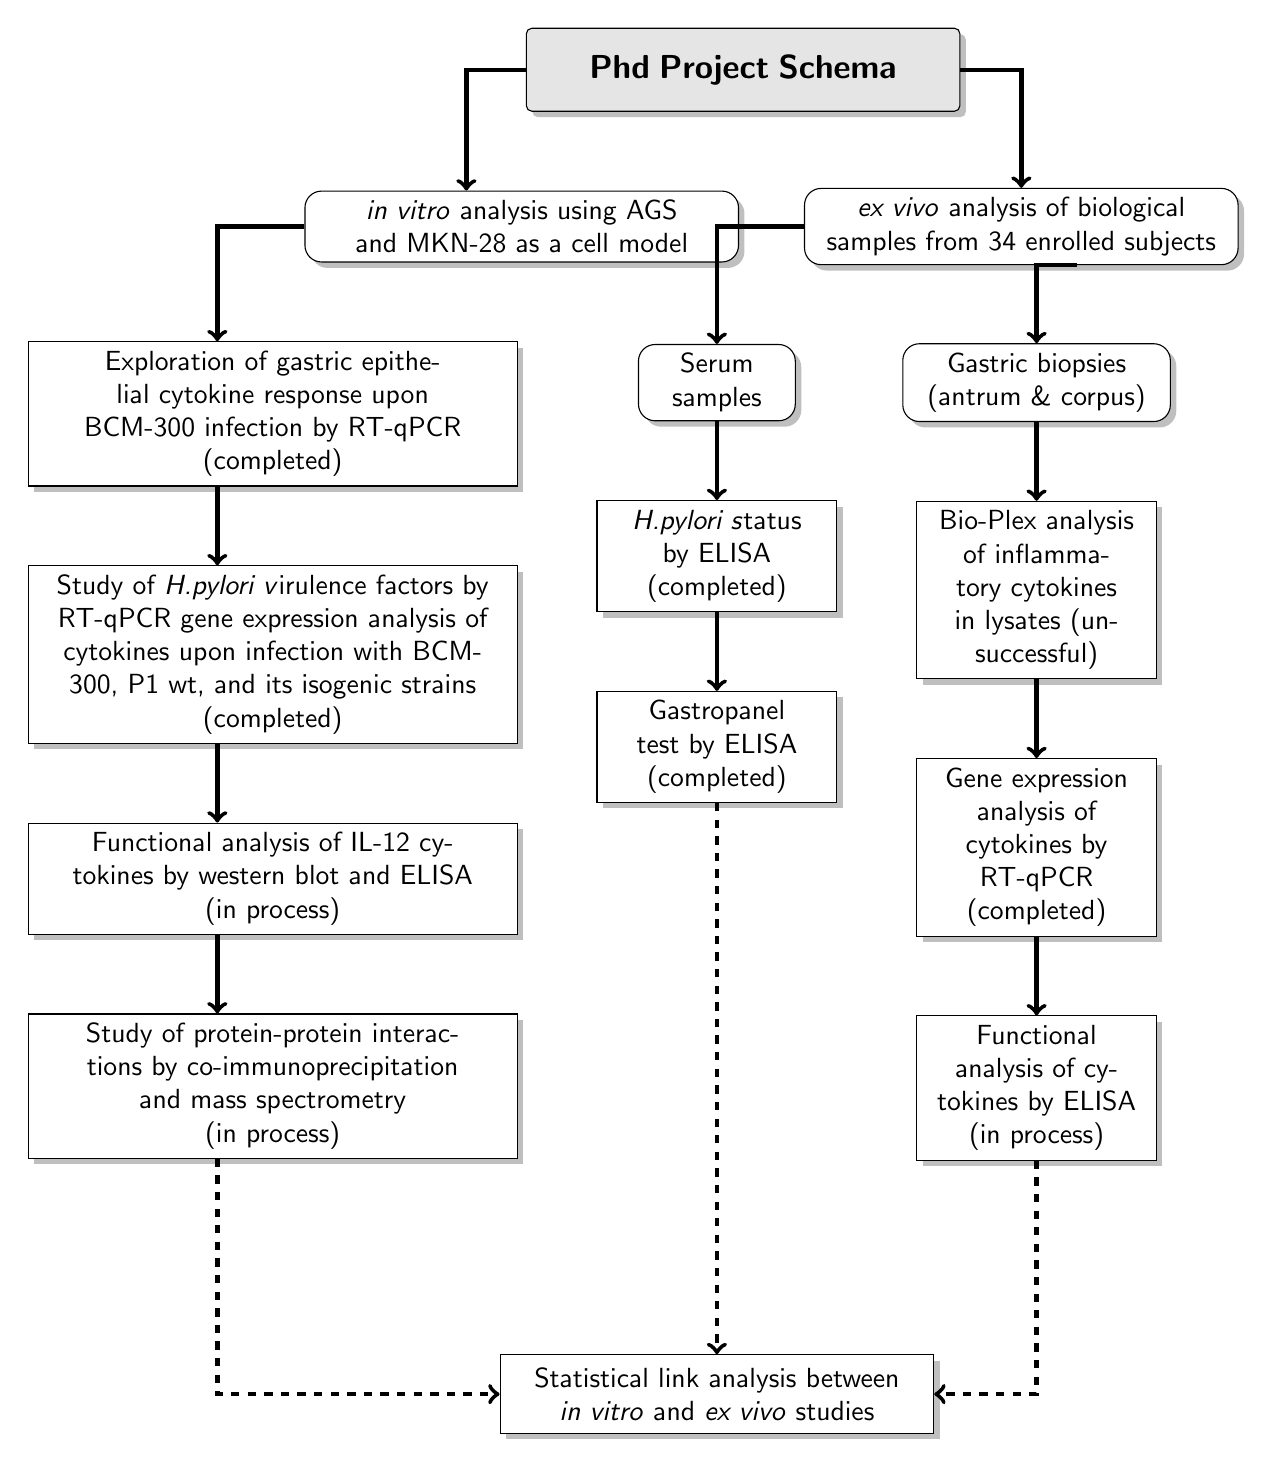
\begin{tikzpicture}
\node [root,text centered, minimum height=30pt,text width=15em] (start) {\textbf{{\large Phd Project Schema}}};
\node [level 2, below=1cm of start, xshift=-80pt] (c1) {{\textit{in vitro} analysis using AGS and MKN-28 as a cell model}};
\node [level 2, right= of c1, xshift=-5pt] (c2) {{\textit{ex vivo} analysis of biological samples from 34 enrolled subjects}};
\node [level 2, text width=5em, below = 1cm of c2, xshift=-110pt] (c21){Serum samples};
\node [level 2, right = of c21, xshift=10pt, text width=9em] (c22){Gastric biopsies (antrum \& corpus)};
% The second level, relatively positioned nodes
\begin{scope}[every node/.style={level 3}]
% branch of exploration of cytokines
\node [below =1cm of c1, xshift=-90pt, text width=17em] (c11){Exploration of gastric epithelial cytokine response upon BCM-300 infection by RT-qPCR\\ (completed)};
\node [below =1cm of c11,text width=17em] (c12) {Study of \species {H.pylori} virulence factors by RT-qPCR gene expression analysis of cytokines upon infection with BCM-300, P1 wt, and its isogenic strains\\ (completed)};
\node [below =1cm of c12, text width=17em] (c13) {Functional analysis of IL-12 cytokines by western blot and ELISA\\ (in process)};
\node [below =1cm of c13, text width=17em] (c14) {Study of protein-protein interactions by co-immunoprecipitation and mass spectrometry\\ (in process)};
% below branch of serum samplees
\node [below =1cm of c21] (c211) {\species {H.pylori} status by ELISA\\ (completed) };
\node [below =1cm of c211] (c212) {Gastropanel test by ELISA\\ (completed)};
% below branch of gastric biopsies
\node [below =1cm of c22] (c221) {Bio-Plex analysis of inflammatory cytokines in lysates (unsuccessful)};
\node [below =1cm of c221] (c222) {Gene expression analysis of cytokines by RT-qPCR\\ (completed)};
\node [below =1cm of c222] (c223) {Functional analysis of cytokines by ELISA\\  (in process)};
% final block
\node [below =7cm of c212, text width=15em, align=center] (c213) {Statistical link analysis between \textit{in vitro} and \textit{ex vivo} studies };
\end{scope}
% draw lines from the start node (c1)
\draw [->, ultra thick] (start.west) -| ([xshift=-2em]c1.north) ; % to in vitro
\draw [->, ultra thick] (start.east) -| (c2.north) ; % to ex vivo
% draw lines of in vitro branch (4 branches)
%\foreach \value in {1,...,4}
\draw [->, ultra thick] (c1.west)  -| ([xshift=-2em]c11.north) ;
\draw [->, ultra thick] ([xshift=-2em]c11.south)  -| ([xshift=-2em]c12.north) ;
\draw [->, ultra thick] ([xshift=-2em]c12.south)  -| ([xshift=-2em]c13.north) ;
\draw [->, ultra thick] ([xshift=-2em]c13.south)  -| ([xshift=-2em]c14.north) ;
% draw lines of ex vivo gastric biopsies branch (3 branches)
\draw [->, ultra thick] ([xshift=20pt]c2.south)  -| (c22.north) ; % to gastric bx
\draw [->, ultra thick] (c2.west)  -| (c21.north) ; % to serum samples
% lines from gastric biopsies to its children
%\draw [->, ultra thick] (c22.east) -- ([xshift=1em]c22.east)  |- (c221.east) ;
\draw [->, ultra thick] (c22.south) -| (c221.north) ;
\draw [->, ultra thick] (c221.south) -| (c222.north) ;
\draw [->, ultra thick] (c222.south) -| (c223.north) ;
% lines from serum samples to its children
\draw [->, ultra thick] (c21.south) -| (c211.north) ;
\draw [->, ultra thick] (c211.south) -| (c212.north) ;
% lines to final block of the chart
\draw [->, ultra thick, dashed] (c212.south) -| (c213.north) ;
\draw [->, ultra thick, dashed] ([xshift=-2em]c14.south) |- (c213.west) ;
\draw [->, ultra thick, dashed] (c223.south) |- (c213.east) ;
\end{tikzpicture}

\end{document}
